\section{Discussion}
\label{sec:discussion}

\subsection{SHAP Explainability}

SHAP (SHapley Additive exPlanations) values were computed using TreeExplainer for Random Forest and XGBoost on 500 test samples. The top features by mean $|SHAP|$ value reveal the decision logic.

\begin{table}[H]
\centering
\caption{Top 10 Features by Mean $|SHAP|$ (Random Forest)}
\label{tab:shap_rf}
\begin{tabular}{lr}
\toprule
\textbf{Feature} & \textbf{Mean $|SHAP|$} \\
\midrule
swap\_intensity & 0.0659 \\
has\_noise\_model & 0.0536 \\
n\_swaps & 0.0455 \\
n\_insertions & 0.0308 \\
n\_two\_qubit\_gates & 0.0121 \\
gate\_ins\_intensity & 0.0119 \\
circuit\_depth & 0.0114 \\
normalized\_entropy & 0.0104 \\
dp\_error\_rate & 0.0097 \\
prob\_cv & 0.0095 \\
\bottomrule
\end{tabular}
\end{table}

\begin{table}[H]
\centering
\caption{Top 10 Features by Mean $|SHAP|$ (XGBoost)}
\label{tab:shap_xgb}
\begin{tabular}{lr}
\toprule
\textbf{Feature} & \textbf{Mean $|SHAP|$} \\
\midrule
swap\_intensity & 2.0406 \\
n\_swaps & 1.2898 \\
has\_noise\_model & 0.5908 \\
n\_insertions & 0.4951 \\
normalized\_entropy & 0.2842 \\
n\_two\_qubit\_gates & 0.2486 \\
prob\_cv & 0.2131 \\
n\_single\_qubit\_gates & 0.1879 \\
exec\_time\_sec & 0.0773 \\
outcome\_ratio & 0.0747 \\
\bottomrule
\end{tabular}
\end{table}

\begin{figure}[H]
\centering
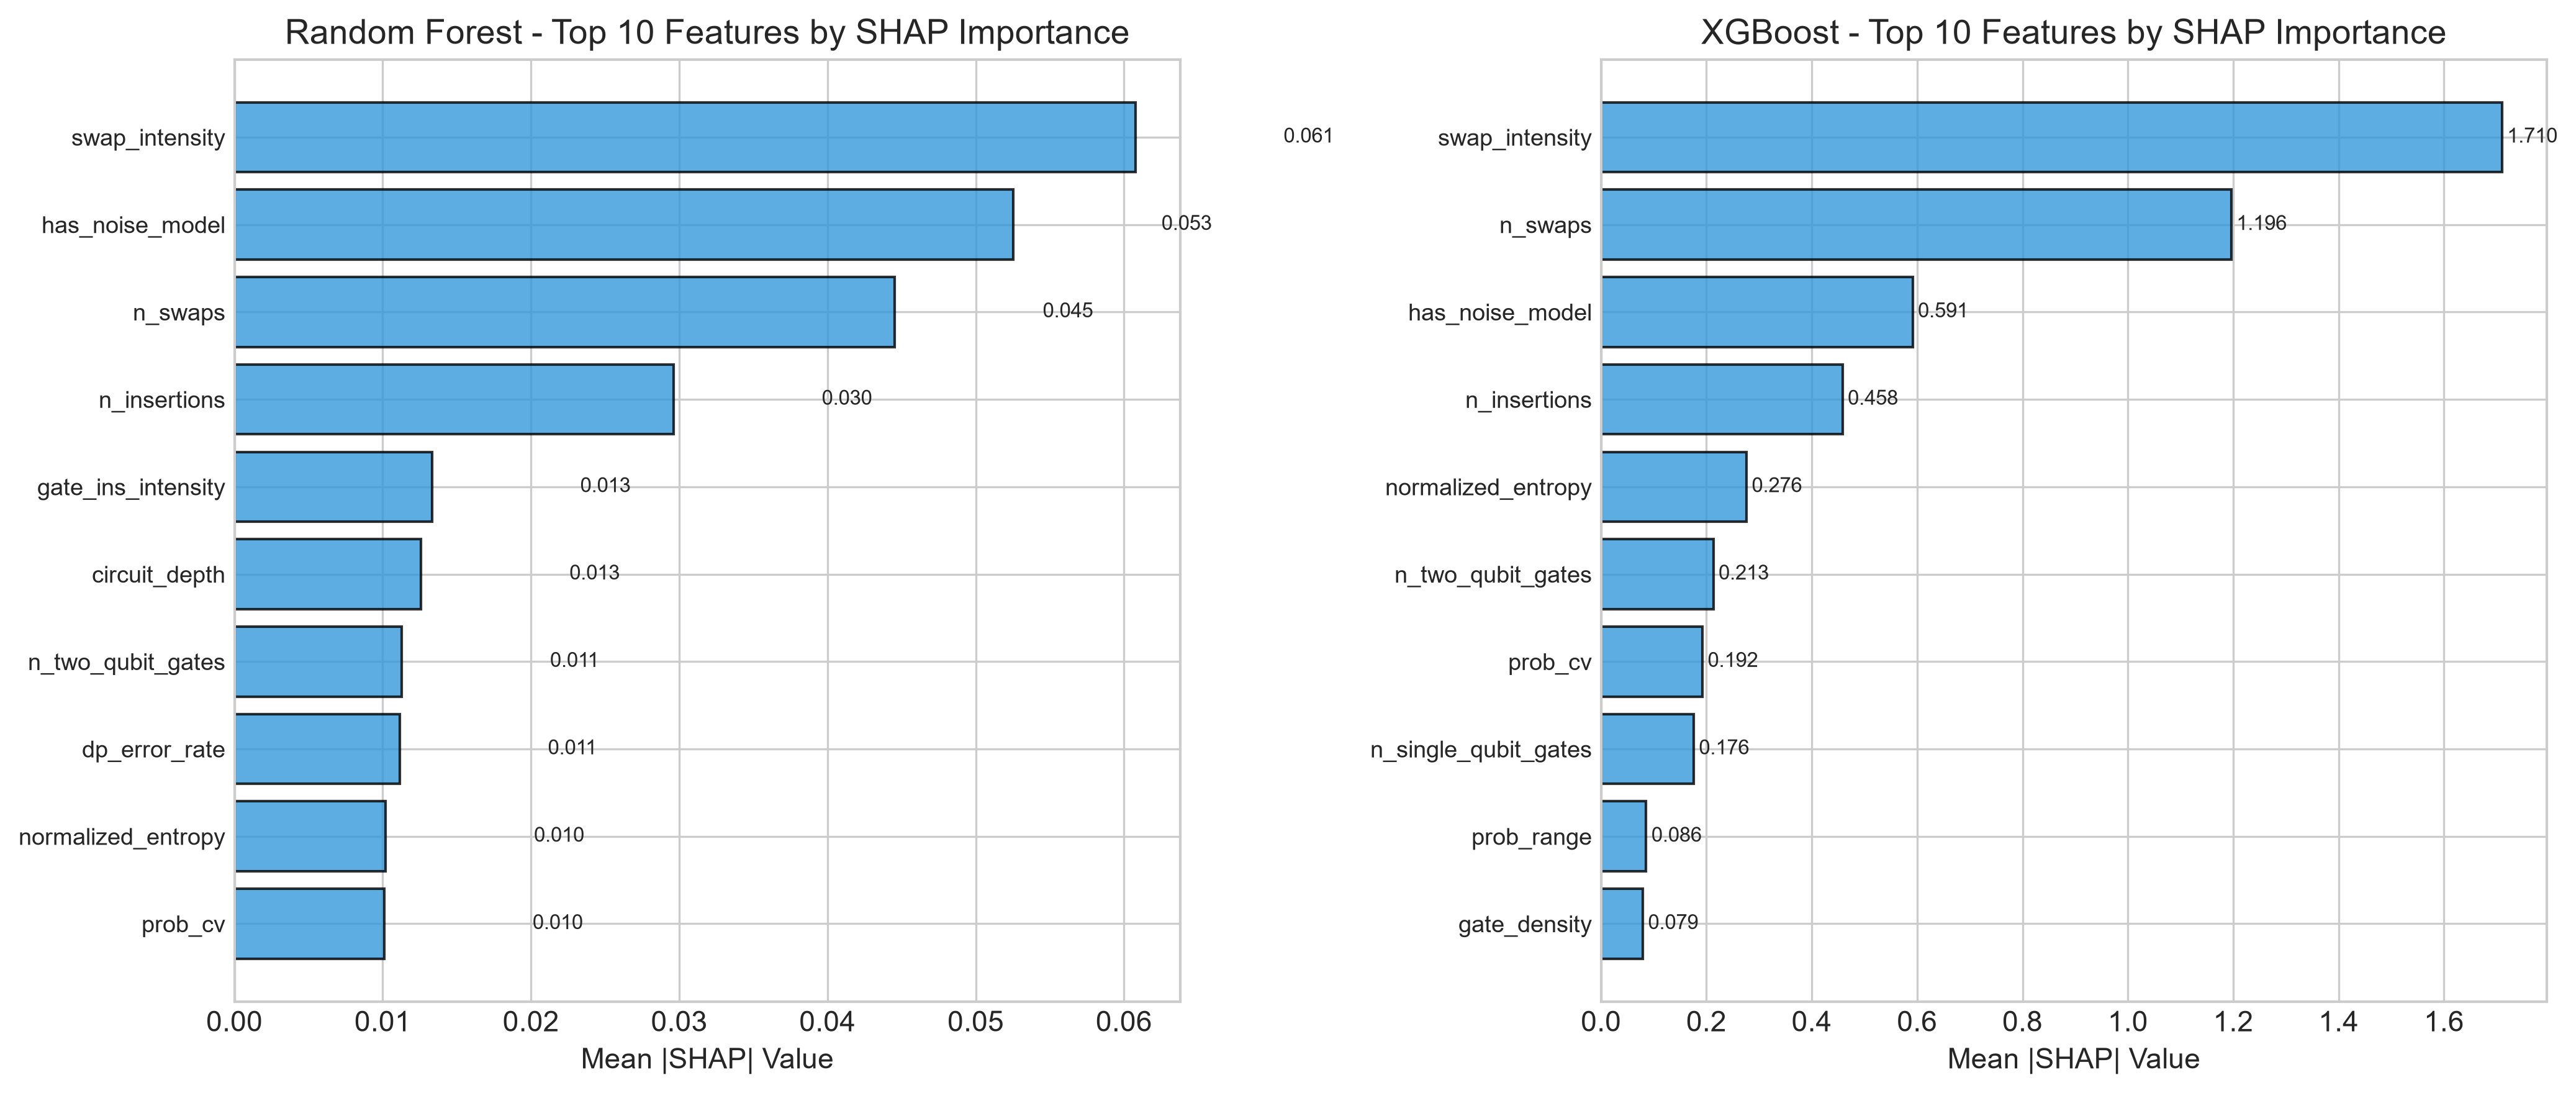
\includegraphics[width=\textwidth]{figures/shap_importance.png}
\caption{Top 10 features by mean $|SHAP|$ for Random Forest and XGBoost.}
\label{fig:shap_importance}
\end{figure}

\textbf{Critical finding:} The dominant features for both models are \textbf{attack-specific simulator parameters}:
\begin{itemize}
    \item \texttt{swap\_intensity}, \texttt{n\_swaps} $\rightarrow$ only non-zero for swap\_injection
    \item \texttt{gate\_ins\_intensity}, \texttt{n\_insertions} $\rightarrow$ only non-zero for gate\_insertion
    \item \texttt{dp\_error\_rate} $\rightarrow$ only non-zero for depolarizing\_noise
    \item \texttt{mt\_flip\_prob} $\rightarrow$ only non-zero for measurement\_tampering
    \item \texttt{has\_noise\_model} $\rightarrow$ binary indicator: 0 for clean, 1 for any attack
\end{itemize}

The first non-attack-specific feature (\texttt{normalized\_entropy}) ranks 5th for XGBoost (SHAP 0.276) and 9th for RF (SHAP 0.010). This confirms the models primarily learn the simulator's attack configuration encoding rather than generalizable attack signatures.

\subsection{Feature-Group Ablation}
\label{sec:ablation}

Leave-one-group-out ablation quantifies the contribution of each semantic feature group. The model is retrained after removing each group.

\begin{table}[H]
\centering
\caption{Feature-Group Ablation: Accuracy and Macro-F1 Drop from Baseline (verified from latest run)}
\label{tab:ablation}
\begin{tabular}{lcccccc}
\toprule
\textbf{Group} & \textbf{N} & \multicolumn{2}{c}{\textbf{XGBoost}} & \multicolumn{2}{c}{\textbf{Random Forest}} & \textbf{SVM-RBF} \\
\cmidrule(lr){3-4} \cmidrule(lr){5-6} \cmidrule(lr){7-7}
 & & $\Delta$Acc & $\Delta$F1 & $\Delta$Acc & $\Delta$F1 & $\Delta$Acc \\
\midrule
attack\_specific\_params & 11 & \textbf{14.2\%} & \textbf{17.4\%} & \textbf{16.1\%} & \textbf{19.4\%} & 5.3\% \\
circuit\_structure & 12 & 5.3\% & 6.7\% & 5.9\% & 7.4\% & \textbf{32.2\%} \\
output\_distribution & 11 & -0.7\%* & -0.9\%* & -0.5\%* & -0.6\%* & -2.8\%* \\
purity\_diversity & 8 & 0.6\% & 0.8\% & 0.2\% & 0.2\% & 0.3\% \\
entropy\_features & 2 & 0.5\% & 0.6\% & 0.3\% & 0.4\% & 1.1\% \\
timing & 1 & 0.7\% & 0.8\% & 0.4\% & 0.5\% & 0.3\% \\
\bottomrule
\end{tabular}
\end{table}

*Negative drop = slight improvement (within noise). Drop values shown as percentage points.

\begin{figure}[H]
\centering
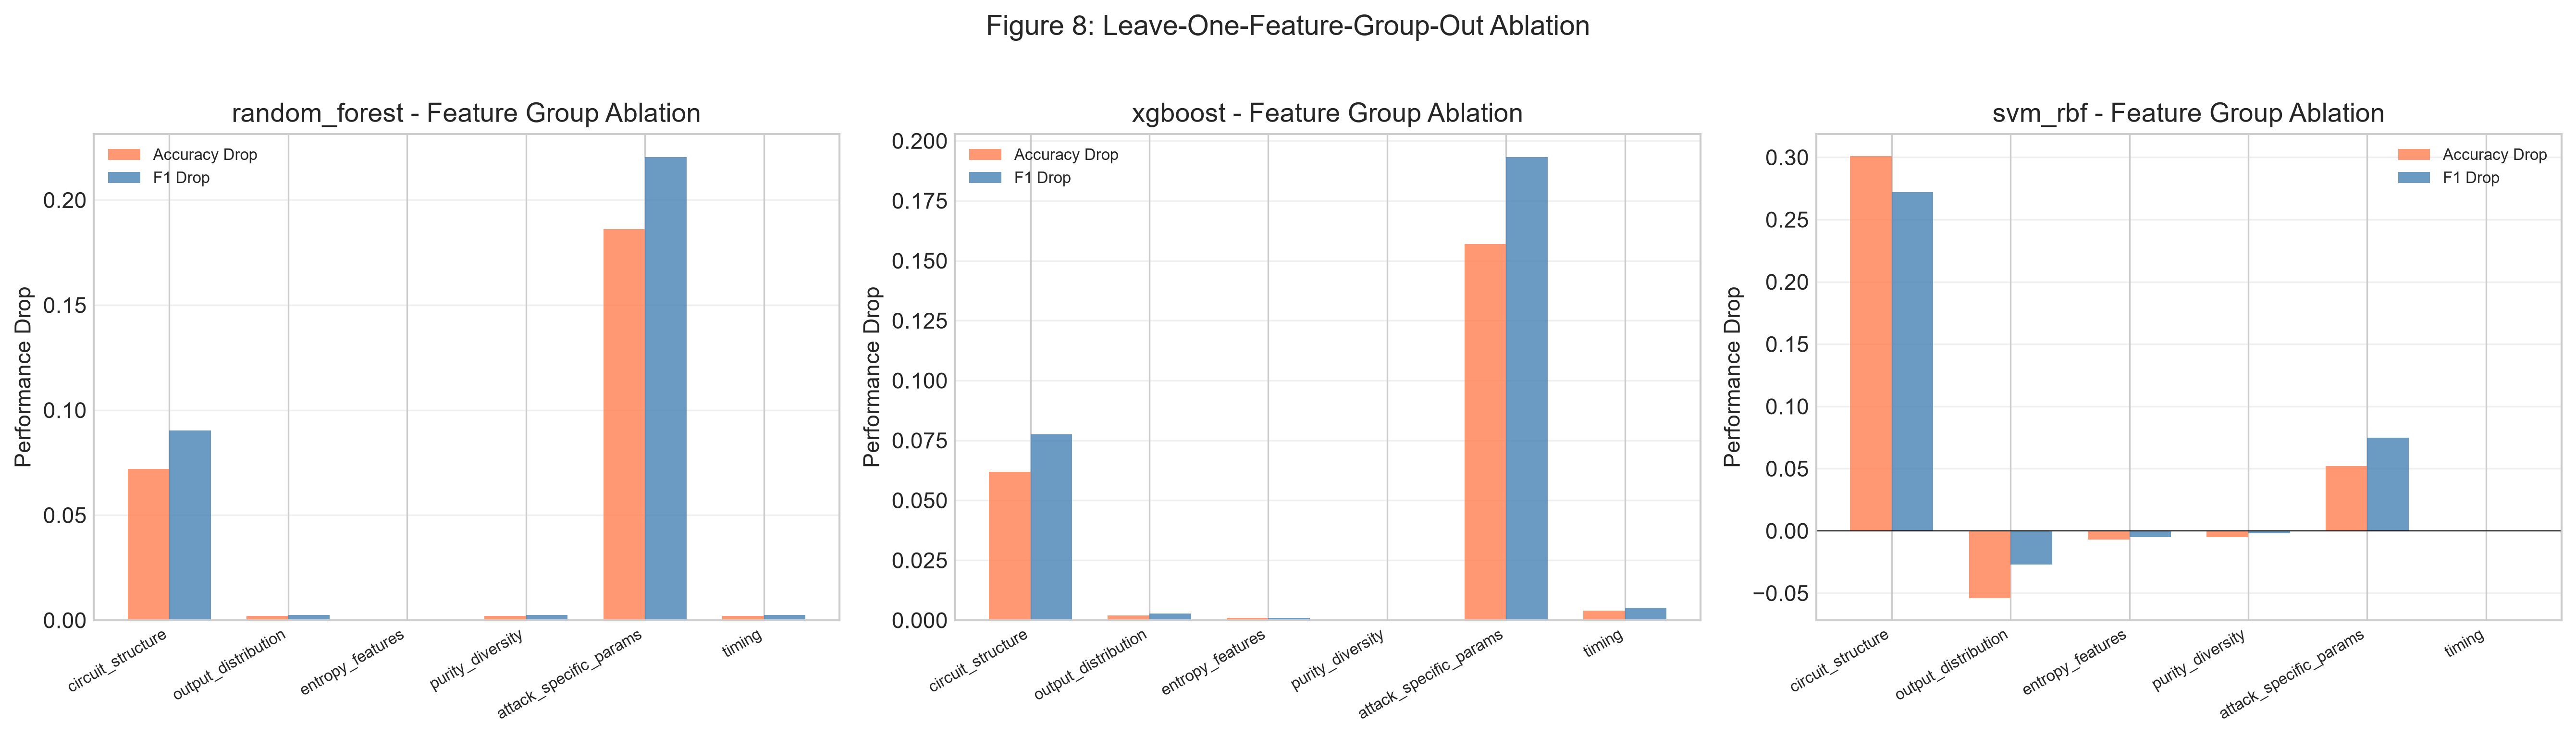
\includegraphics[width=\textwidth]{figures/ablation.png}
\caption{Leave-one-feature-group-out ablation for all three classifiers. Bars show drop in accuracy (coral) and macro-F1 (blue) when each group is removed.}
\label{fig:ablation}
\end{figure}

\textbf{Interpretation:}
\begin{enumerate}
    \item \textbf{Tree models (RF, XGBoost):} Attack-specific parameters are overwhelmingly important (14-19\% drop in accuracy, 17-22\% in F1). Circuit structure is secondary (5-7\%). Removing output distribution slightly \emph{improves} performance (negative drop within noise), suggesting these features add noise. All other groups have negligible impact.
    \item \textbf{SVM-RBF:} Circuit structure is most important (32\% accuracy drop). Attack-specific parameters contribute only 5\%. This suggests SVM relies on geometric separation in the circuit-structure feature space.
    \item \textbf{Leakage confirmation:} The 14-19\% accuracy drop from removing attack-specific parameters directly quantifies the label leakage. Without these features, tree models lose their primary decision signal and drop to ~80\% accuracy (RF) and ~81\% (XGBoost). A controlled experiment removing \texttt{has\_noise\_model} alone showed minimal impact on tree models but hurt SVM-RBF, confirming that the attack-specific parameters (not just the binary indicator) are the primary leakage vector.
\end{enumerate}

\subsection{Error Analysis}

\begin{table}[H]
\centering
\caption{Most Common Misclassifications (Test Set, n=2,000)}
\label{tab:errors}
\begin{tabular}{llll}
\toprule
\textbf{Model} & \textbf{True} $\rightarrow$ \textbf{Pred} & \textbf{Count} & \textbf{Pattern} \\
\midrule
XGBoost & measurement\_tampering $\rightarrow$ pulse\_level\_attack & 23 & Noise similarity \\
XGBoost & pulse\_level\_attack $\rightarrow$ measurement\_tampering & 12 & Noise similarity \\
XGBoost & depolarizing\_noise $\rightarrow$ pulse\_level\_attack & 3 & Noise similarity \\
Random Forest & measurement\_tampering $\rightarrow$ pulse\_level\_attack & 23 & Noise similarity \\
Random Forest & pulse\_level\_attack $\rightarrow$ measurement\_tampering & 12 & Noise similarity \\
Random Forest & gate\_insertion $\rightarrow$ swap\_injection & 5 & Structural similarity \\
SVM-RBF & Widespread confusion across all attack types & -- & Low discriminative power \\
\bottomrule
\end{tabular}
\end{table}

The primary confusion is between \texttt{measurement\_tampering} and \texttt{pulse\_level\_attack}, both of which introduce noise-like disturbances. The secondary confusion is \texttt{gate\_insertion} $\leftrightarrow$ \texttt{swap\_injection}, both structural modifications.

\subsection{Comparison to Reference Paper Targets}

\begin{table}[H]
\centering
\caption{Comparison: QAD Results vs. Reference Paper Targets}
\label{tab:comparison}
\begin{tabular}{llcc}
\toprule
\textbf{Aspect} & \textbf{Metric} & \textbf{QAD (Ours)} & \textbf{Paper Target} \\
\midrule
Dataset & Type & Quantum circuit attacks & BB84 eavesdropping \\
Dataset & Samples & 10,000 (1M avail) & 24,000 \\
Dataset & Features & 45 (42 + 3 one-hot) & 63 temporal-QBER \\
Dataset & Classes & 8 (1 clean + 7 circuit) & 8 (1 normal + 7 QKD) \\
Model & Best & XGBoost & XGBoost \\
Model & Accuracy & 95.75\% & 88.01\% \\
Model & Macro-F1 & 0.9463 & 0.8803 \\
Binary & FNR (XGB) & 0.00\% & N/A \\
Binary & Threshold (11\%) & N/A & 25.82\% \\
Binary & CUSUM & N/A & 78.99\% \\
Binary & XGBoost & N/A & 88.01\% \\
\bottomrule
\end{tabular}
\end{table}

\textbf{Key conclusion:} The QAD results are \textbf{not comparable} to the paper's targets. The higher accuracy on QAD stems from label leakage via attack-specific parameters, not superior attack detection. The paper's 88.01\% is on a harder problem (temporal-QBER with overlapping channel conditions across classes, no attack-specific simulator parameters).